$B%7%_%e%l!<%7%g%s(B4

%energy history
\begin{figure}[htbp]
 \begin{center}
 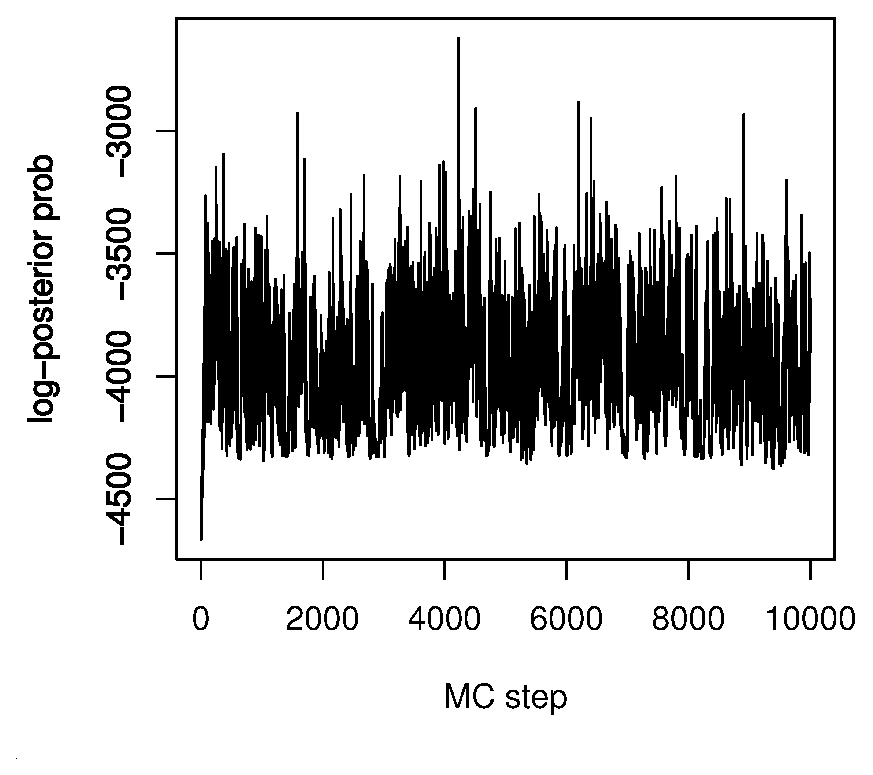
\includegraphics[width=10cm,height=5cm]{./fig/simu_4/energy_history.eps}
\caption{simulation 4: $BBP?tL`EY4X?t$NA+0\(B}
\label{fig:simu_4_log-posterior}
 \end{center}
\end{figure}
%%histgrams of delta
%\begin{figure}
% \begin{tabular}{ccc}
% 
%  \begin{minipage}{0.33\hsize}
%   \begin{center}
%    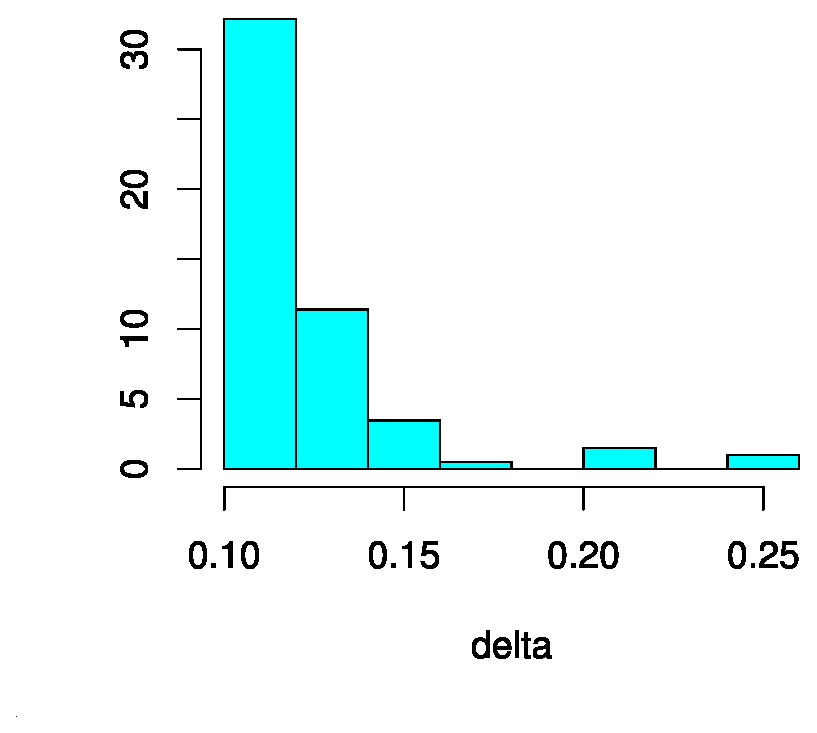
\includegraphics[width=5cm]{./fig/simu_4/hist_delta1.eps}
%   \end{center}
%   \caption{simu4: $\delta_{1}$ distribution}
%   \label{simu_4_hist_delta1}
%  \end{minipage}
%  \begin{minipage}{0.33\hsize}
%   \begin{center}
%    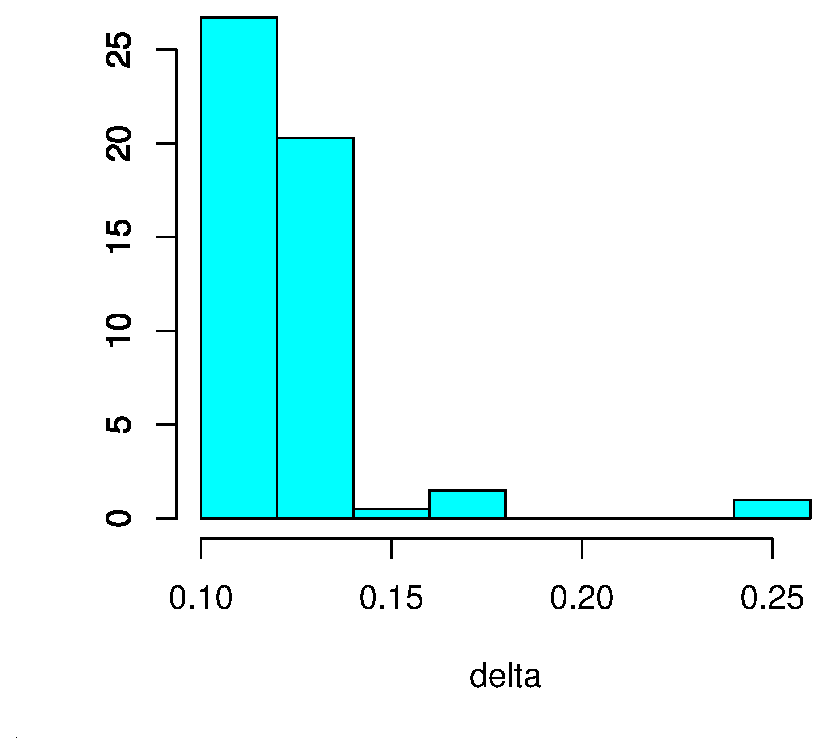
\includegraphics[width=5cm]{./fig/simu_4/hist_delta2.eps}
%   \end{center}
%   \caption{simu4: $\delta_{2}$ distribution}
%   \label{simu_4_hist_delta2}
%
%  \end{minipage}
%  \begin{minipage}{0.33\hsize}
%   \begin{center}
%    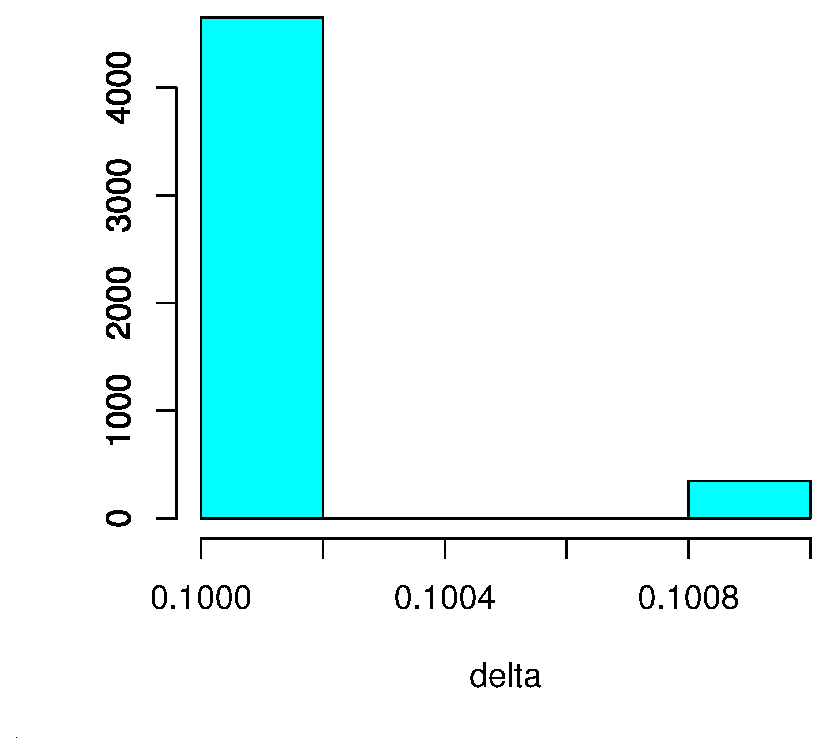
\includegraphics[width=5cm]{./fig/simu_4/hist_delta3.eps}
%   \end{center}
%   \caption{simu4: $\delta_{3}$ distribution}
%   \label{simu_4_hist_delta3}
%  \end{minipage}
%
%\\
%%histgrams of delta
%  \begin{minipage}{0.33\hsize}
%   \begin{center}
%    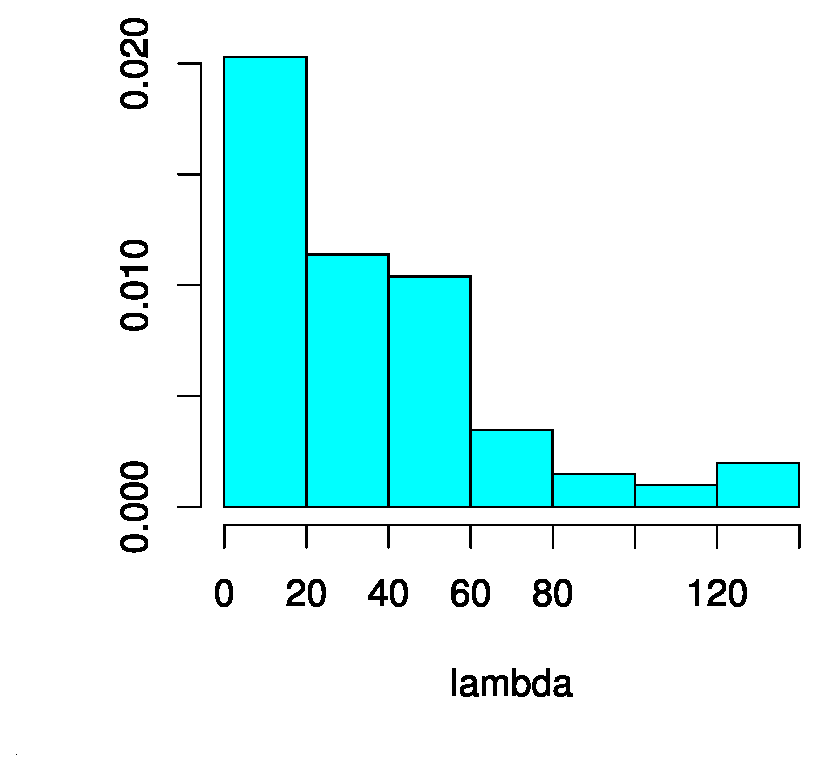
\includegraphics[width=5cm]{./fig/simu_4/hist_lambda1.eps}
%   \end{center}
%   \caption{simu4: $\lambda_{1}$ distribution}
%   \label{simu_4_hist_lambda1}
%  \end{minipage}
%  \begin{minipage}{0.33\hsize}
%   \begin{center}
%    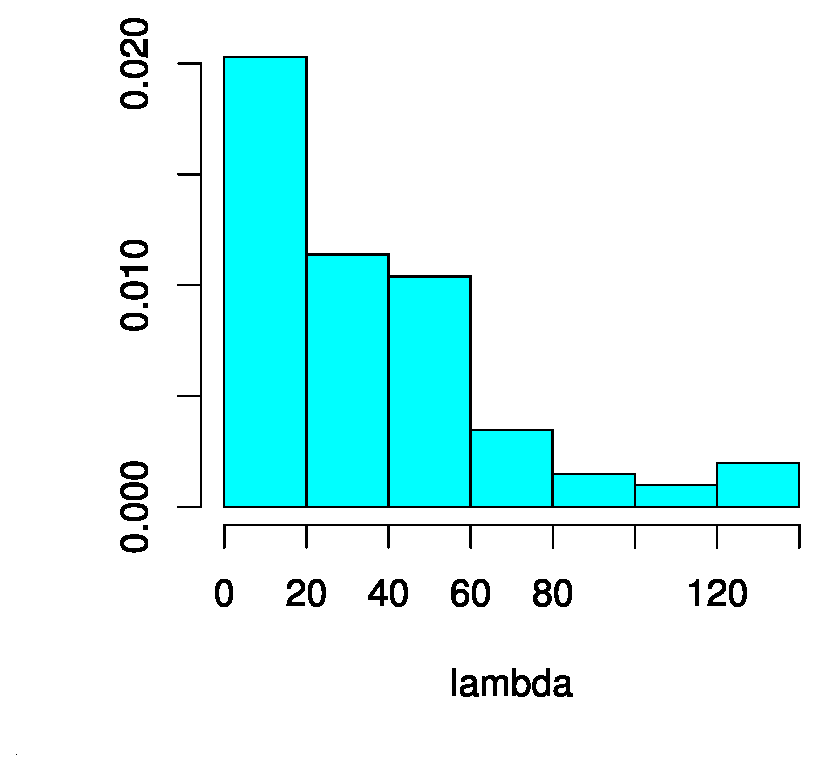
\includegraphics[width=5cm]{./fig/simu_4/hist_lambda1.eps}
%   \end{center}
%   \caption{simu4: $\lambda_{2}$ distribution}
%   \label{simu_4_hist_lambda2}
%  \end{minipage}
%  \begin{minipage}{0.33\hsize}
%   \begin{center}
%    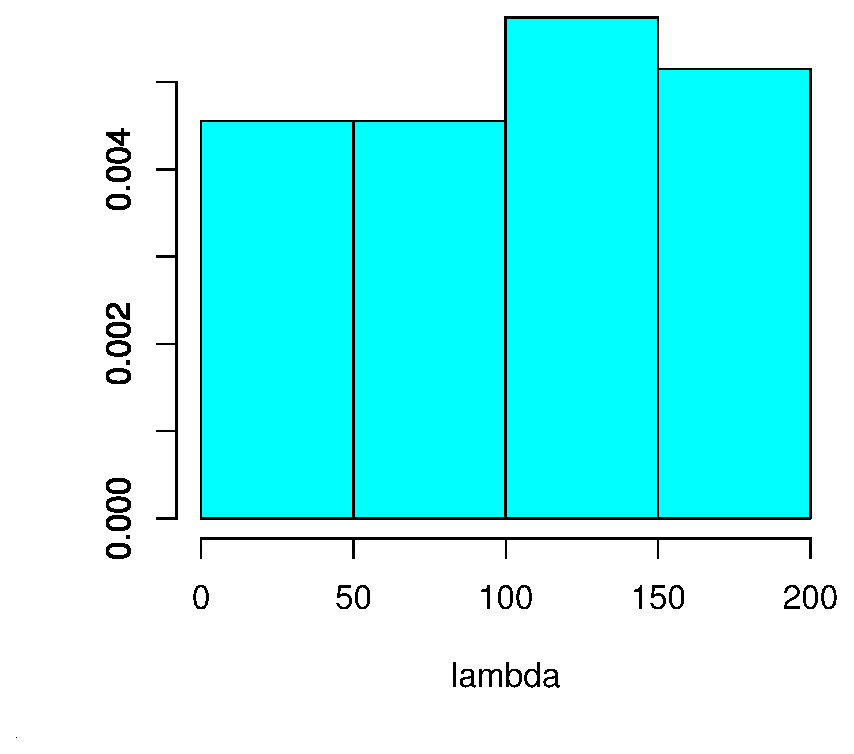
\includegraphics[width=5cm]{./fig/simu_4/hist_lambda3.eps}
%   \end{center}
%   \caption{simu4: $\lambda_{3}$ distribution}
%   \label{simu_4_hist_lambda3}
%  \end{minipage}
% \end{tabular}
%%\caption{$B;v8eJ,I[(B}
%\end{figure}
%
%\clearpage
%


\begin{figure} [h]
 \centering
 %hist of delta
 \subfigure[$\delta_{1}$]{
 \label{fig_a} 
 \resizebox{5cm}{4cm}{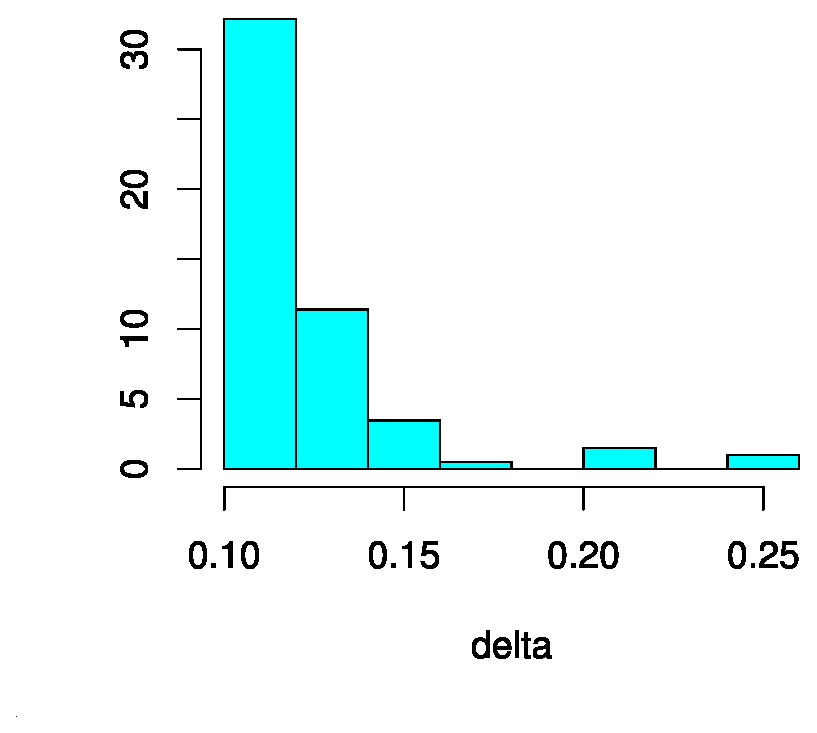
\includegraphics{./fig/simu_4/hist_delta1.eps}}}
 \subfigure[$\delta_{2}$]{
 \label{fig_b} 
 \resizebox{5cm}{4cm}{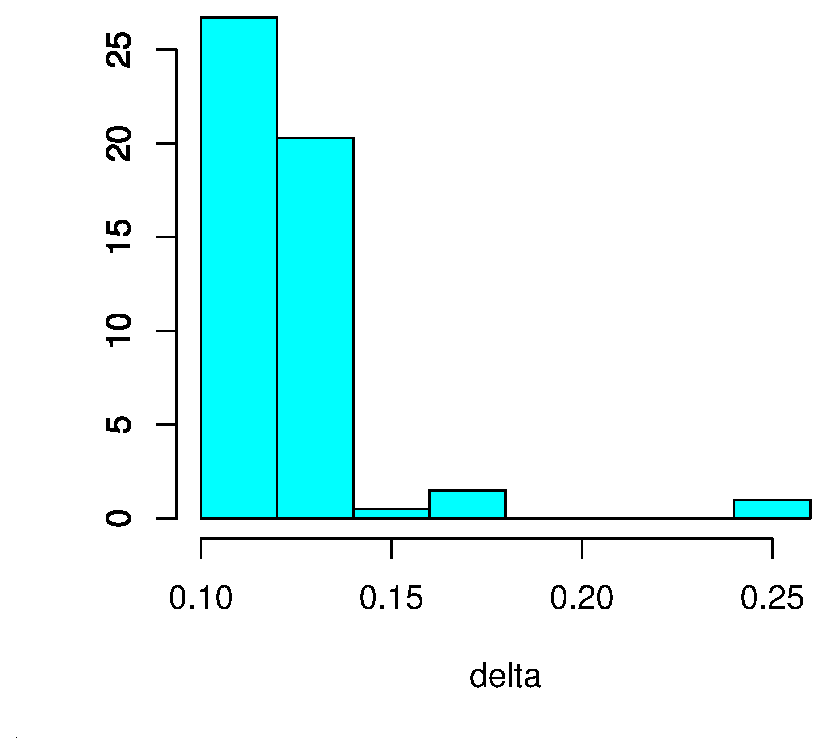
\includegraphics{./fig/simu_4/hist_delta2.eps}}}
 \subfigure[$\delta_{3}$]{
 \label{fig_c}
 \resizebox{5cm}{4cm}{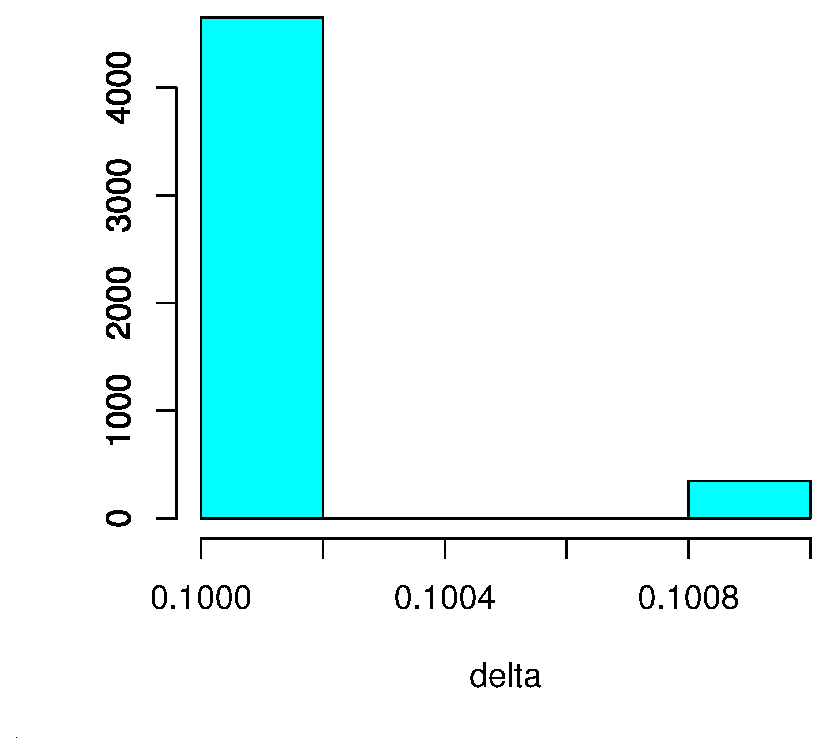
\includegraphics{./fig/simu_4/hist_delta3.eps}}}
 \label{fig_total}


 %hist of lambda
 \subfigure[$\lambda_{1}$]{
 \label{fig_a} 
 \resizebox{5cm}{4cm}{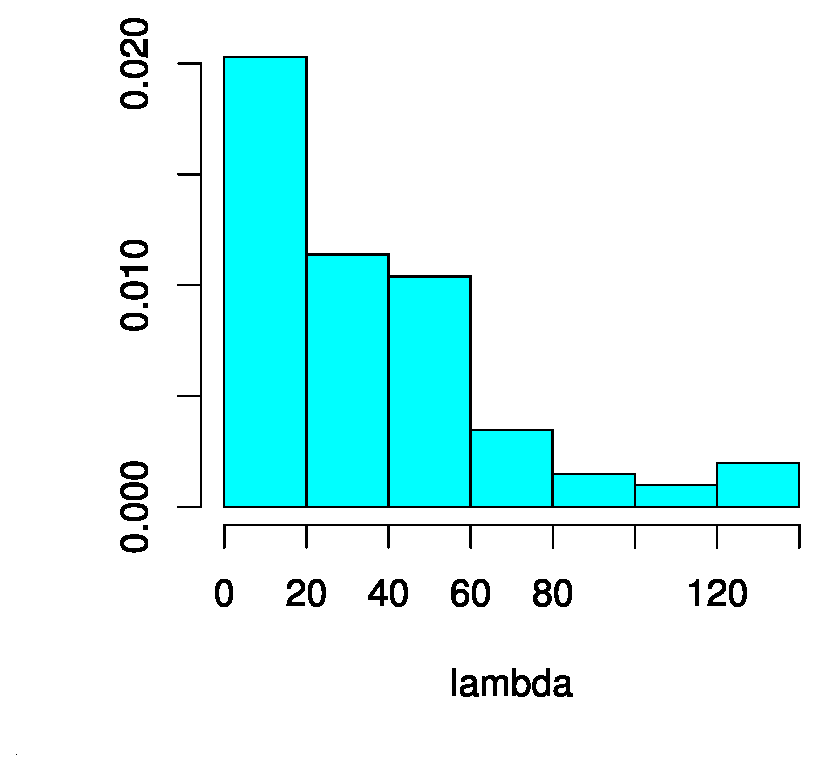
\includegraphics{./fig/simu_4/hist_lambda1.eps}}}
 \subfigure[$\lambda_{2}$]{
 \label{fig_b} 
 \resizebox{5cm}{4cm}{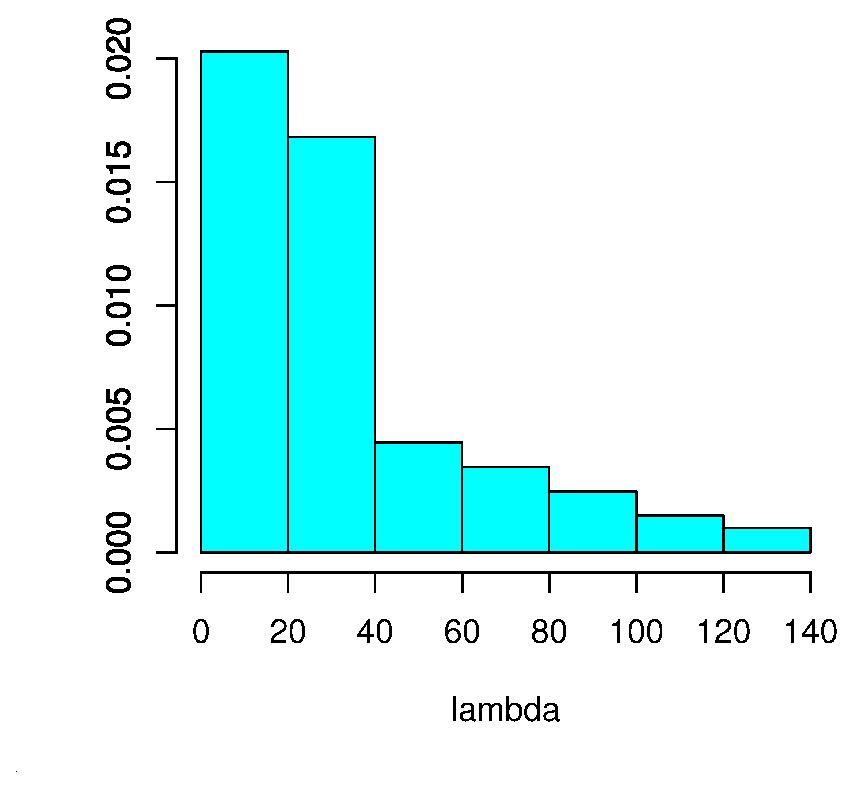
\includegraphics{./fig/simu_4/hist_lambda2.eps}}}
 \subfigure[$\lambda_{3}$]{
 \label{fig_c}
 \resizebox{5cm}{4cm}{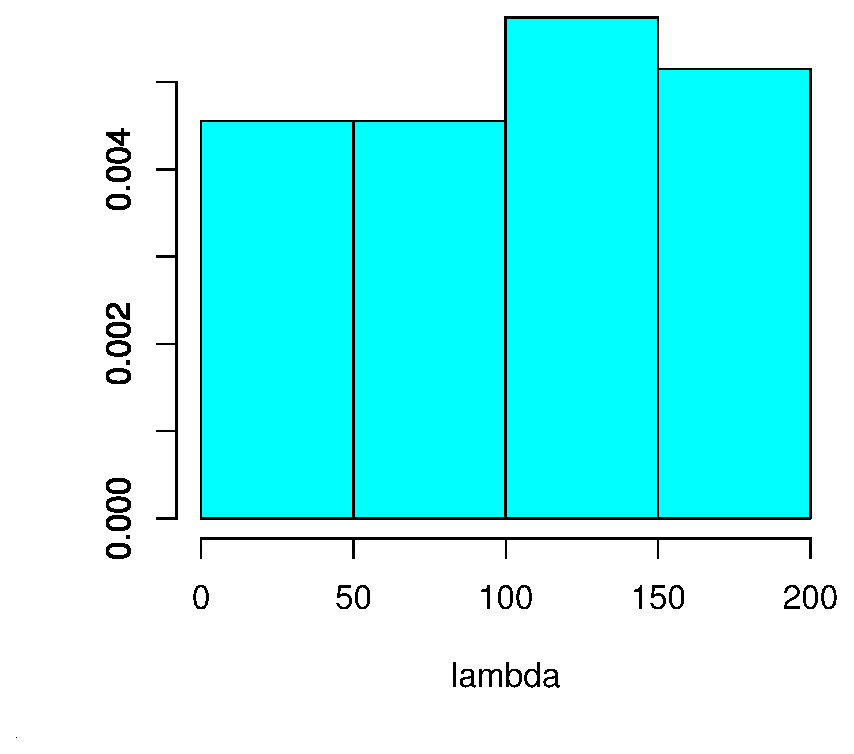
\includegraphics{./fig/simu_4/hist_lambda3.eps}}}
 \label{fig_total}
\caption{simulation 4: $B3F%Q%i%a!<%?$N%R%9%H%0%i%`(B}
\label{fig:sim4_histgram}
\end{figure}


\clearpage